\documentclass[11pt]{article}
\usepackage[utf8]{inputenc}
\usepackage[T1]{fontenc}
\usepackage{amsmath}
\usepackage{amssymb}
\usepackage{multicol}
\usepackage{geometry}
\usepackage{tikz}
\usepackage{enumitem}
\usepackage{xcolor}
\usepackage{titlesec}
\usetikzlibrary{shadows}
\usepackage{graphicx}
\usepackage{ragged2e}

% Configurações de layout
\geometry{a4paper, left=1cm, right=1cm, top=0.5cm, bottom=1.2cm}
\setlength{\columnseprule}{0.4pt}

% Cores para títulos
\titleformat{\section}{\normalfont\Large\bfseries\color{blue}}{\thesection}{1em}{}
\titleformat{\subsection}{\normalfont\large\bfseries\color{red}}{\thesubsection}{1em}{}

\title{\textcolor{blue}{Terceiro Trimestre: Aprofundamento em Matemática  \\ Análise Combinatória: Princípios e Técnicas de Contagem}}
\author{Professor: Jefferson}
\date{}

\begin{document}

\maketitle
\vspace{-1cm}

\begin{center}
\large{Nome: \underline{\hspace{8cm}} \quad Turma: \underline{\hspace{3cm}}}
\end{center}

\begin{multicols}{2}

\section*{Habilidade da Aula}

% CAIXA COLORIDA COM A HABILIDADE
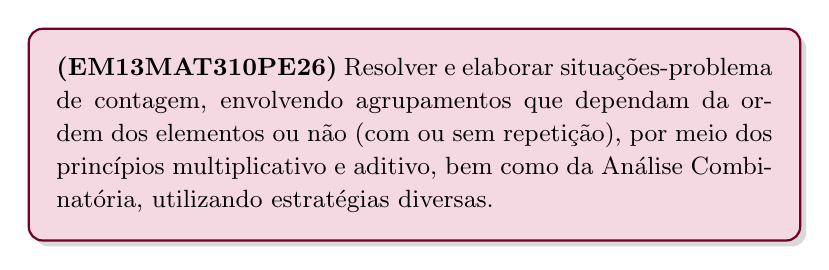
\begin{tikzpicture}
\node[rectangle, 
      fill=purple!15, 
      rounded corners=5pt, 
      inner sep=10pt, 
      draw=purple!60!black, 
      thick,
      drop shadow={opacity=0.3},
      text width=0.75\linewidth,
      align=justify] 
{
\small
\textbf{(EM13MAT310PE26)} Resolver e elaborar situações-problema de contagem, envolvendo agrupamentos que dependam da ordem dos elementos ou não (com ou sem repetição), por meio dos princípios multiplicativo e aditivo, bem como da Análise Combinatória, utilizando estratégias diversas.
};
\end{tikzpicture}


\section*{1. Princípios Fundamentais}

\subsection*{Princípio Multiplicativo}

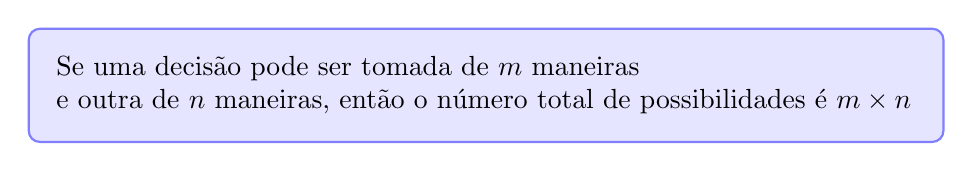
\begin{tikzpicture}
\node[rectangle, fill=blue!10, rounded corners, inner sep=10pt, draw=blue!50, thick, text width=0.9\linewidth, align=justify] {
Se uma decisão pode ser tomada de $m$ maneiras \\ 
e outra de $n$ maneiras, então o número total de possibilidades é $m \times n$
};
\end{tikzpicture}

\vspace{5mm}

\textbf{Exemplo:}
Quanta combinações são possíveis com 3 camisetas e 2 calças?
\[
3 \times 2 = 6 \text{ combinações diferentes}
\]

\subsection*{Princípio Aditivo}

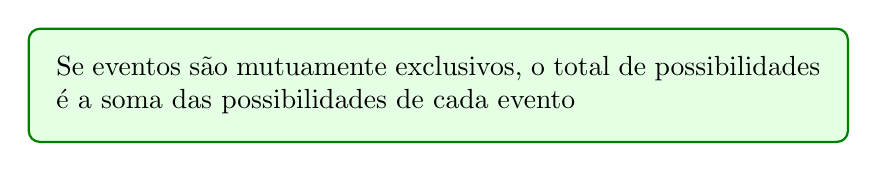
\begin{tikzpicture}
\node[rectangle, fill=green!10, rounded corners, inner sep=10pt, draw=green!50!black, thick, text width=0.8\linewidth, align=justify] {
Se eventos são mutuamente exclusivos, o total de possibilidades é a soma das possibilidades de cada evento
};
\end{tikzpicture}

\vspace{5mm}

\textbf{Exemplo:}
Temos 4 livros de Matemática e 3 de Física. De quantas maneiras podemos escolher um livro?
\[
4 + 3 = 7 \text{ maneiras}
\]

\section*{2. Agrupamentos e Arranjos}

\subsection*{Permutação Simples}

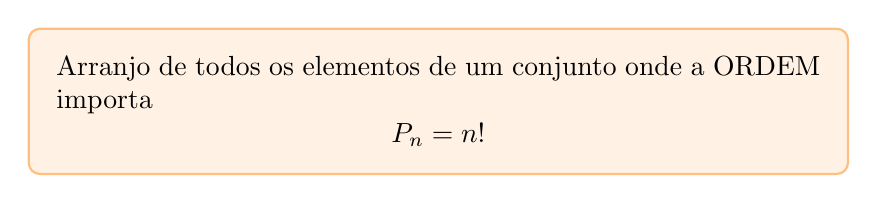
\begin{tikzpicture}
\node[rectangle, fill=orange!10, rounded corners, inner sep=10pt, draw=orange!50, thick, text width=0.8\linewidth, align=justify] {
Arranjo de todos os elementos de um conjunto onde a ORDEM importa
\[
P_n = n!
\]
};
\end{tikzpicture}

\vspace{5mm}

\textbf{Exemplo:}
De quantas maneiras 4 pessoas podem se sentar em um banco?
\[
P_4 = 4! = 4 \times 3 \times 2 \times 1 = 24
\]

\subsection*{Permutação com Repetição}

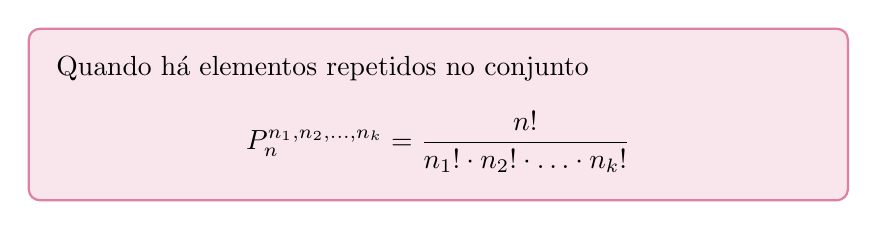
\begin{tikzpicture}
\node[rectangle, fill=purple!10, rounded corners, inner sep=10pt, draw=purple!50, thick, text width=0.8\linewidth, align=justify] {
Quando há elementos repetidos no conjunto
\[
P_n^{n_1,n_2,\ldots,n_k} = \frac{n!}{n_1! \cdot n_2! \cdot \ldots \cdot n_k!}
\]
};
\end{tikzpicture}

\vspace{5mm}

\textbf{Exemplo:}
Quantos anagramas tem a palavra "BANANA"?
\[
P_6^{3,2} = \frac{6!}{3! \cdot 2!} = \frac{720}{6 \times 2} = 60
\]

\section*{3. Combinações e Arranjos}

\subsection*{Arranjo Simples}

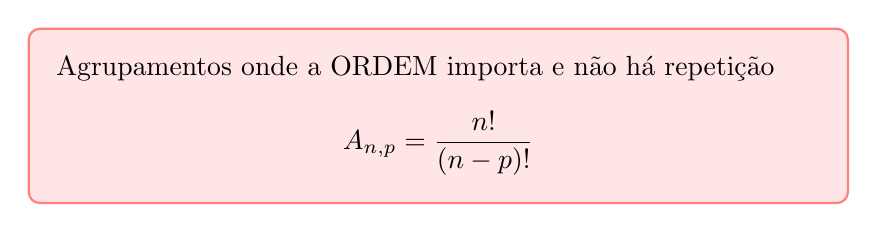
\begin{tikzpicture}
\node[rectangle, fill=red!10, rounded corners, inner sep=10pt, draw=red!50, thick, text width=0.8\linewidth, align=justify] {
Agrupamentos onde a ORDEM importa e não há repetição
\[
A_{n,p} = \frac{n!}{(n-p)!}
\]
};
\end{tikzpicture}

\vspace{5mm}

\textbf{Exemplo:}
Quantos números de 2 algarismos distintos formamos com {1,2,3,4}?
\[
A_{4,2} = \frac{4!}{2!} = \frac{24}{2} = 12
\]

\subsection*{Combinação Simples}


\begin{tikzpicture}
\node[rectangle, fill=teal!10, rounded corners, inner sep=10pt, draw=teal!50, thick, text width=0.8\linewidth, align=justify] {
Agrupamentos onde a ordem NÃO importa
\[
C_{n,p} = \binom{n}{p} = \frac{n!}{p!(n-p)!}
\]
};
\end{tikzpicture}

\vspace{5mm}

\textbf{Exemplo:}
Quantas comissões de 3 pessoas formamos com 5 pessoas?
\[
C_{5,3} = \frac{5!}{3!2!} = \frac{120}{6 \times 2} = 10
\]

\section*{4. Tabela Comparativa}

\begin{center}
\begin{tabular}{|c|c|c|}
\hline
\textbf{Tipo} & \textbf{Ordem importa?} & \textbf{Fórmula} \\
\hline
Permutação & Sim & $n!$ \\
\hline
Arranjo & Sim & $\frac{n!}{(n-p)!}$ \\
\hline
Combinação & Não & $\frac{n!}{p!(n-p)!}$ \\
\hline
\end{tabular}
\end{center}

\section*{5. Exercícios - Nível Básico}

\begin{enumerate}[leftmargin=*]
\item Quantos números de 3 algarismos distintos podemos formar com os dígitos 1, 2, 3, 4, 5?

\item Uma prova tem 8 questões, mas o aluno deve escolher 5 para responder. De quantas maneiras ele pode fazer essa escolha?

\item Quantos anagramas tem a palavra "MATEMÁTICA"?

\item Em uma sala há 10 homens e 8 mulheres. Quantas comissões de 4 pessoas podemos formar com:
\begin{enumerate}[label=\alph*)]
\item Qualquer pessoa?
\item 2 homens e 2 mulheres?
\item Pelo menos 1 mulher?
\end{enumerate}

\item Quantos números pares de 4 algarismos distintos podemos formar com os dígitos 1, 2, 3, 4, 5, 6?

\item (ENEM) Um restaurante oferece 5 tipos de salada, 3 tipos de prato principal e 4 tipos de sobremesa. De quantas maneiras um cliente pode escolher uma refeição com:
\begin{enumerate}[label=\alph*)]
\item Um item de cada tipo?
\item Apenas prato principal e sobremesa?
\end{enumerate}

\item Quantas diagonais tem um decágono?

\item De quantas maneiras 6 pessoas podem se sentar em torno de uma mesa circular?

\item Uma senha deve conter 4 caracteres: 2 letras (dentre 26) e 2 números (dentre 10). Quantas senhas são possíveis se:
\begin{enumerate}[label=\alph*)]
\item Letras e números podem repetir?
\item Nenhum caractere pode repetir?
\end{enumerate}

\item Quantos são os subconjuntos de um conjunto com 5 elementos?
\end{enumerate}

\section*{6. Exercícios - Nível Intermediário}

\begin{enumerate}[leftmargin=*, start=11]
\item Quantos números ímpares de 4 algarismos distintos existem entre 1000 e 5000?

\item Uma empresa tem 12 funcionários, sendo 7 homens e 5 mulheres. De quantas maneiras podemos formar uma comissão de 5 pessoas com maioria feminina?

\item Quantos anagramas da palavra "PARALELOGRAMO" começam e terminam com vogal?

\item Em um torneio com 8 times, quantos jogos são realizados se cada time joga contra todos os outros exatamente uma vez?

\item Quantos números naturais de 1 a 1000 são divisíveis por 3 ou por 5?

\item De quantas maneiras podemos distribuir 8 livros diferentes entre 3 estudantes, se cada estudante deve receber pelo menos 2 livros?

\item Quantos triângulos podem ser formados unindo-se os vértices de um octógono?

\item Quantas soluções naturais possui a equação $x + y + z = 12$?

\item Em uma prateleira há 5 livros de Matemática, 4 de Física e 3 de Química, todos diferentes. De quantas maneiras podemos organizá-los se os livros de mesma matéria devem ficar juntos?

\item Quantos números de 5 algarismos possuem pelo menos um dígito par?
\end{enumerate}


\subsection*{Dica Importante}
\begin{center}
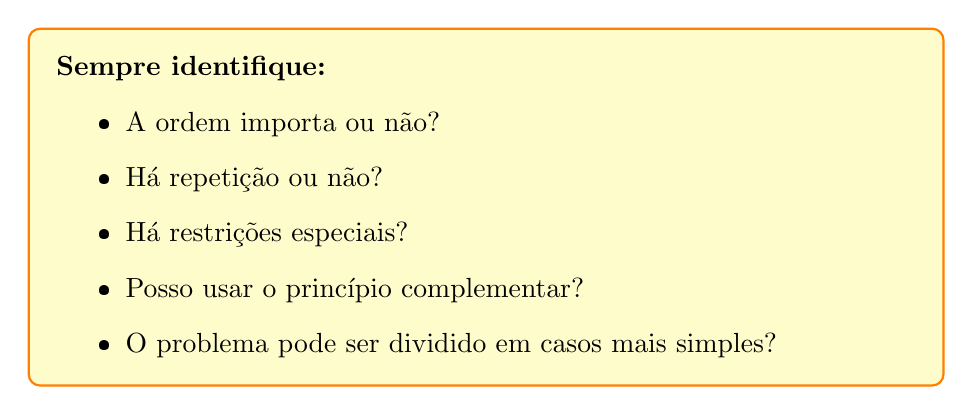
\begin{tikzpicture}
\node[rectangle, fill=yellow!20, rounded corners, inner sep=10pt, draw=orange, thick, text width=0.9\linewidth, align=justify] {
\textbf{Sempre identifique:}
\begin{itemize}
\item A ordem importa ou não?
\item Há repetição ou não?
\item Há restrições especiais?
\item Posso usar o princípio complementar?
\item O problema pode ser dividido em casos mais simples?
\end{itemize}
};
\end{tikzpicture}
\end{center}


\end{multicols}

\end{document}
